\documentclass[11pt]{article}
\usepackage[margin=1in]{geometry}
\usepackage{amsmath}
\usepackage{amssymb}
\usepackage{graphicx}
\usepackage{booktabs}
\usepackage{hyperref}
\usepackage{xcolor}


\title{Project 2}
\author{Kaitlyn Anderson, Mary Bergemann, Reed Wiseman}
\date{November 20, 2026}

\begin{document}
\sloppy
\maketitle

\paragraph{Lotka-Volterra Equations Part 1}\\
\begin{align*}
    \frac{dx}{dt} &= \alpha x-\beta xy\\
    \frac{dy}{dt} &= -\gamma y+\delta xy
\end{align*}\\
The Lotka-Volterra equations is a set of two differential equations with an ecological basis. These equations describe the relationship between a predator and prey or a parasite and a host. The function assumes four fixed rates represented by alpha, beta, gamma, and delta. These numbers describe the growth rate of prey, the rate at which predators kill prey, the rate predators die, and the rate predator population increases due to the fact they are eating the prey, respectively. 

\paragraph{Rössler Attraction Part 1}
\begin{align*}
    \frac{dx}{dt} &= -y-x\\
    \frac{dy}{dt} &= x+ay\\
    \frac{dz}{dt} &= b +z(x-c)\\
\end{align*}

The Rössler Attractor is a third order ordinary differential equation that is separated out into the three equations seen above. Each parameter (a,b,c) is varied, and each one gives a different result including causing the system to converge towards a fixed point, periodic endpoint, or infinity. This system contains two fixed points, one in the middle that is unstable and settles into a chaotic attractor and one on the outside of the region of the attractor. The trajectory starts with the point in the middle of the attractor and continues along its path until it exits the x-y plane where it approaches the second point. This repeats in cycles and ultimately describes the behavior of a chaotic attractor. 

\begin{figure}[h]
    \centering
    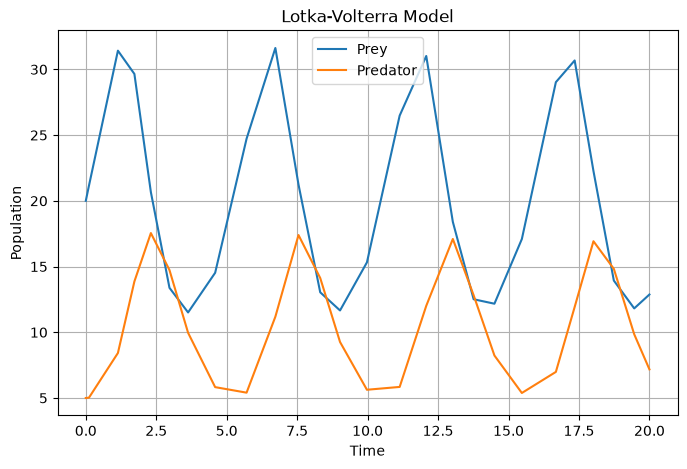
\includegraphics[width=0.5\linewidth]{LV1.png}
    \caption{LV Graph: Parameters \alpha = 1.0, \beta = 0.1, \gamma = 1.5, \delta = 0.075}
    \label{fig:placeholder}
\end{figure}
\begin{figure}[h]
    \centering
    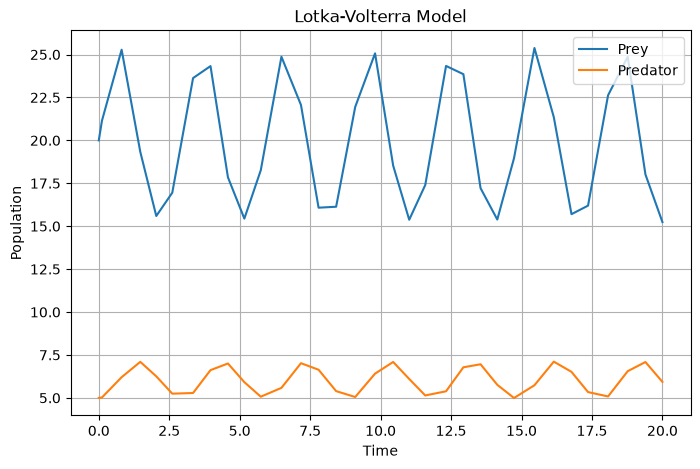
\includegraphics[width=0.5\linewidth]{LV20.png}
    \caption{LV Graph: Parameters \alpha = 3.0, \beta = 0.5, \gamma = 1.5, \delta = 0.075}
    \label{fig:placeholder}
\end{figure}
\begin{figure}[h]
    \centering
    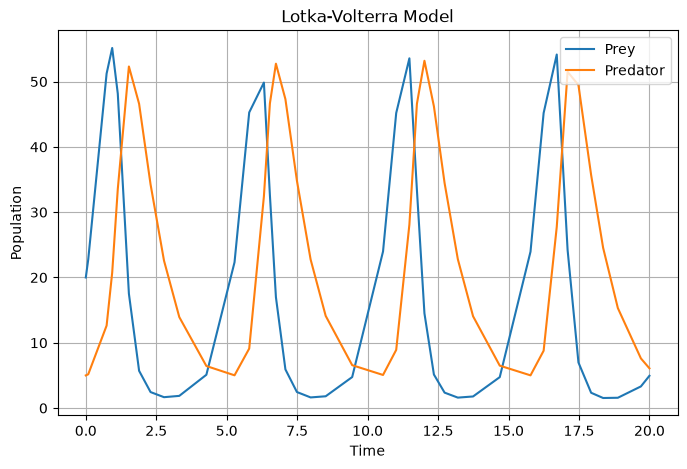
\includegraphics[width=0.5\linewidth]{LV30.png}
    \caption{LV Graph: Parameters \alpha = 2.0, \beta = 0.1, \gamma = 1.0, \delta = 0.065}
    \label{fig:placeholder}
\end{figure}
\clearpage

\begin{figure}[h]
    \centering
    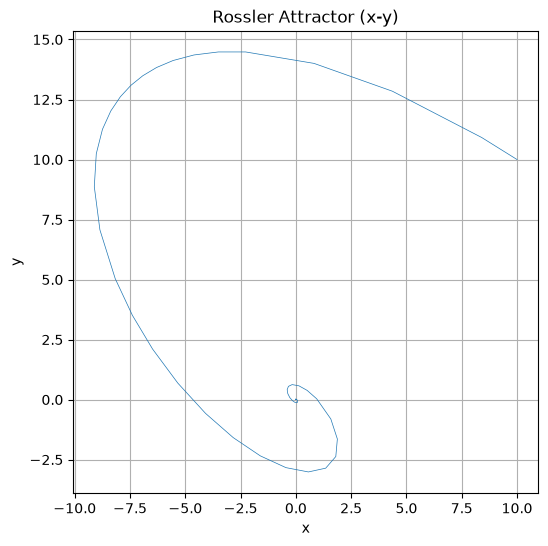
\includegraphics[width=0.5\linewidth]{RA10.png}
    \caption{Rössler Attraction Graph: Parameters a=0.2, b=0.2, c=5.7}
    \label{fig:placeholder}
\end{figure}

\begin{figure}[h]
    \centering
    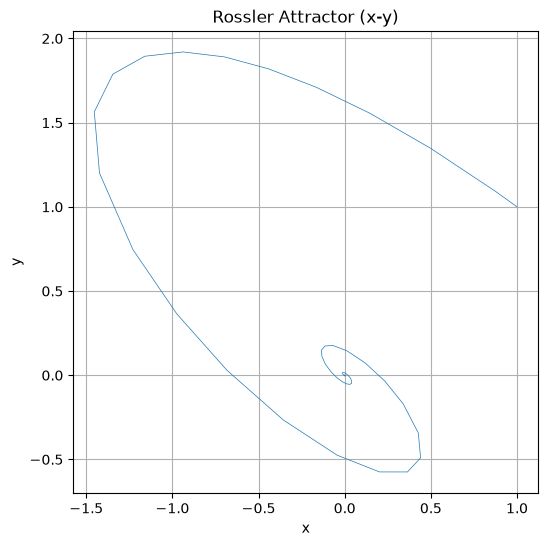
\includegraphics[width=0.5\linewidth]{RA2.png}
    \caption{Rössler Attraction Graph: Parameters a=0.5, b=0.3, c=6.7}
    \label{fig:placeholder}
\end{figure}

\begin{figure}[h]
    \centering
    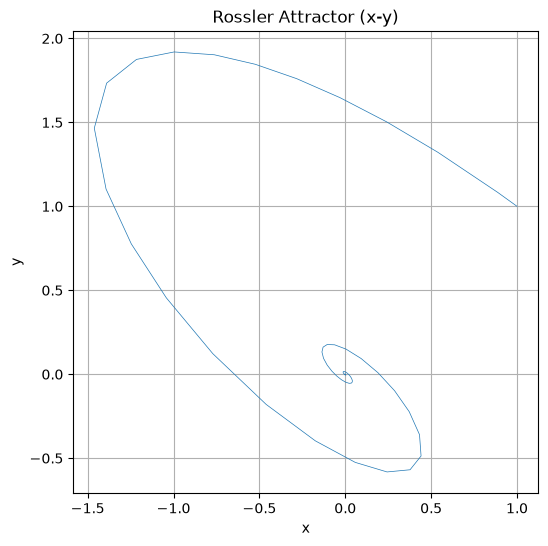
\includegraphics[width=0.5\linewidth]{RA3.png}
    \caption{Rössler Attraction Graph: Parameters a=0.2, b=0.2, c=1.0}
    \label{fig:placeholder}
\end{figure}

\clearpage
\subsection*{Task 3: Numerical Accuracy of the Solver}

To investigate the accuracy of SciPy's
\texttt{solve\_ivp}, we used the logistic equation $f'=f(1-f)$, which has a known exact solution. We selected an initial condition of $f(0)=0.2$ and a final time of $t=5$. We calculated numerical solutions using different relative tolerances (\texttt{rtol}) ranging from $10^{-3}$ to $10^{-10}$, while keeping the absolute tolerance (\texttt{atol}) constant at $10^{-12}$. We then compared each numerical solution with the exact solution at $t=5$ to calculate its absolute error. The results show that decreasing the relative tolerance generally decreases the numerical error, producing a more accurate approximation. However, smaller tolerances generally require the solver to take more steps, increasing computational effort.

\begin{figure}[h]
    \centering
    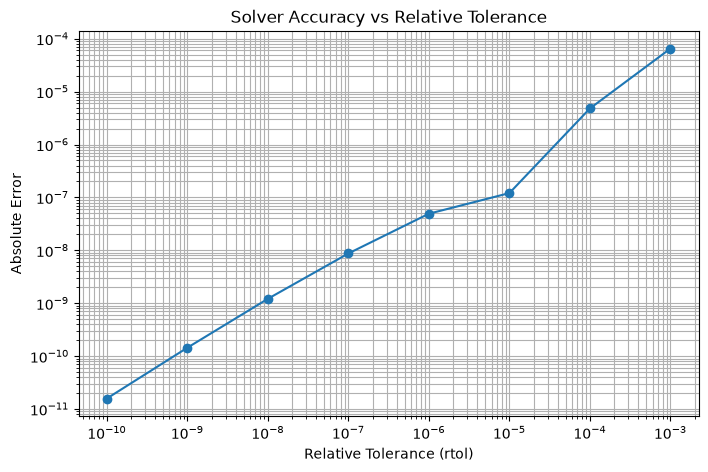
\includegraphics[width=0.5\linewidth]{output.png}
    \caption{Solver Accuracy Vs Relative Tolerance: Parameters $f_0$=0.2, t=(0, 5)}
    \label{fig:placeholder}
\end{figure}

\clearpage
\paragraph{References}-\\
\begin{itemize}
    \item Letellier, Christophe, and Otto E. Rossler. “Rossler Attractor.” Scholarpedia, 3 Oct. 2006, \url{scholarpedia.org/article/R%C3%B6ssler_attractor.}
    \item Wikimedia Foundation. (2026, September 14). List of nonlinear ordinary differential equations. Wikipedia. \url{https://en.wikipedia.org/wiki/List_of_nonlinear_ordinary_differential_equations}
    \item Weisstein, Eric W. "Lotka-Volterra Equations." From MathWorld--A Wolfram Resource. \url{https://mathworld.wolfram.com/Lotka-VolterraEquations.html}
\end{itemize}


\end{document}
